% =========================================================================
% BÀI 10: PHÉP CỘNG TRONG PHẠM VI 10 (CHỦ ĐỀ 3 - TOÁN LỚP 1)
% TOÀN BỘ CÂU HỎI ĐƯỢC VẼ HÌNH MINH HỌA TRỰC QUAN 100% BẰNG TIKZ
% =========================================================================

% --- CÁC HÀM VẼ ĐỒ VẬT, CON VẬT TRỰC QUAN CHO PHÉP CỘNG LỚP 1 ---
\providecommand{\VeQuaTaoDo}[2]{% #1=x, #2=y
  \begin{scope}[shift={(#1,#2)}, scale=0.6]
    \fill[red!85!black] (-0.11,0.08) circle (0.22cm);
    \fill[red!85!black] (0.11,0.08) circle (0.22cm);
    \fill[red!85!black] (0,-0.05) circle (0.24cm);
    \draw[line width=1pt, brown!80!black] (0,0.24) to[out=70,in=-110] (0.06,0.42);
    \fill[green!70!black] (0.05,0.36) to[out=20,in=160] (0.24,0.42) to[out=-120,in=-20] cycle;
  \end{scope}
}

\providecommand{\VeQuaTaoXanh}[2]{% #1=x, #2=y
  \begin{scope}[shift={(#1,#2)}, scale=0.6]
    \fill[green!75!black] (-0.11,0.08) circle (0.22cm);
    \fill[green!75!black] (0.11,0.08) circle (0.22cm);
    \fill[green!75!black] (0,-0.05) circle (0.24cm);
    \draw[line width=1pt, brown!80!black] (0,0.24) to[out=70,in=-110] (0.06,0.42);
    \fill[green!85!black] (0.05,0.36) to[out=20,in=160] (0.24,0.42) to[out=-120,in=-20] cycle;
  \end{scope}
}

\providecommand{\VeChuCa}[3][orange!90!black]{% #1=màu, #2=x, #3=y
  \begin{scope}[shift={(#2,#3)}, scale=0.55]
    \fill[#1] (0,0) ellipse (0.38cm and 0.22cm);
    \fill[#1] (-0.35,0) -- (-0.58,0.2) -- (-0.58,-0.2) -- cycle;
    \fill[white] (0.2,0.06) circle (0.06cm);
    \fill[black] (0.23,0.06) circle (0.03cm);
    \draw[line width=0.6pt, #1!60!black] (0.05,-0.05) arc (-60:60:0.12cm);
  \end{scope}
}

\providecommand{\VeChuCaBoiTrai}[3][cyan!80!blue]{% #1=màu, #2=x, #3=y
  \begin{scope}[shift={(#2,#3)}, scale=0.55, xscale=-1]
    \fill[#1] (0,0) ellipse (0.38cm and 0.22cm);
    \fill[#1] (-0.35,0) -- (-0.58,0.2) -- (-0.58,-0.2) -- cycle;
    \fill[white] (0.2,0.06) circle (0.06cm);
    \fill[black] (0.23,0.06) circle (0.03cm);
    \draw[line width=0.6pt, #1!60!black] (0.05,-0.05) arc (-60:60:0.12cm);
  \end{scope}
}

\providecommand{\VeVienKeo}[3][magenta!80!red]{% #1=màu, #2=x, #3=y
  \begin{scope}[shift={(#2,#3)}, scale=0.58]
    \fill[#1] (-0.28,0) circle (0.12cm);
    \fill[#1] (0.28,0) circle (0.12cm);
    \draw[fill=#1, draw=orange!80!black, line width=0.8pt, rounded corners=3pt] (-0.22,-0.16) rectangle (0.22,0.16);
    \draw[white, line width=0.9pt] (-0.1,-0.14) -- (0.1,0.14);
  \end{scope}
}

\providecommand{\VeChuChimDau}[2]{% #1=x, #2=y
  \begin{scope}[shift={(#1,#2)}, scale=0.55]
    \fill[cyan!85!blue] (0,0.1) ellipse (0.26cm and 0.2cm);
    \fill[cyan!95!black] (0.18,0.22) circle (0.15cm);
    \fill[orange!95!black] (0.32,0.22) -- (0.45,0.19) -- (0.32,0.15) -- cycle;
    \fill[white] (0.22,0.25) circle (0.04cm);
    \fill[black] (0.24,0.25) circle (0.02cm);
    \fill[blue!80!black] (-0.22,0.1) -- (-0.45,0.18) -- (-0.38,0.04) -- cycle;
  \end{scope}
}

\providecommand{\VeChuChimBay}[2]{% #1=x, #2=y
  \begin{scope}[shift={(#1,#2)}, scale=0.55]
    \fill[orange!90!red] (0,0.1) ellipse (0.26cm and 0.18cm);
    \fill[orange!95!black] (-0.18,0.22) circle (0.14cm);
    \fill[yellow!90!black] (-0.31,0.22) -- (-0.43,0.19) -- (-0.31,0.15) -- cycle;
    \fill[white] (-0.22,0.25) circle (0.04cm);
    \fill[black] (-0.24,0.25) circle (0.02cm);
    \fill[red!80!black] (0.05,0.15) -- (0.2,0.48) -- (-0.08,0.2) -- cycle;
  \end{scope}
}

\providecommand{\VeChuVit}[2]{% #1=x, #2=y
  \begin{scope}[shift={(#1,#2)}, scale=0.58]
    \fill[yellow!90!orange] (0,0) ellipse (0.32cm and 0.22cm);
    \fill[yellow!95!orange] (0.22,0.22) circle (0.16cm);
    \fill[orange!90!black] (0.36,0.22) -- (0.52,0.18) -- (0.36,0.14) -- cycle;
    \fill[black] (0.27,0.25) circle (0.035cm);
    \fill[orange!85!black] (-0.25,0.08) -- (-0.42,0.2) -- (-0.35,0) -- cycle;
  \end{scope}
}

\providecommand{\VeBongHoaNho}[3][magenta!80!red]{% #1=màu hoa, #2=x, #3=y
  \begin{scope}[shift={(#2,#3)}, scale=0.55]
    \foreach \a in {0,72,144,216,288} {
      \fill[#1] (\a:0.18) circle (0.12cm);
    }
    \fill[yellow!95!orange] (0,0) circle (0.1cm);
  \end{scope}
}

% =========================================================================
% PHẦN 1: TRẮC NGHIỆM LỰA CHỌN (12 CÂU)
% =========================================================================
\textbf{Phần 1. Trắc nghiệm lựa chọn}
\setcounterpageref{ex}{0}

% --- CÂU 1 ---
\begin{ex} %[1D3N10]
Quan sát hai đĩa táo dưới đây. Hỏi có tất cả bao nhiêu quả táo?
\begin{center}
\begin{tikzpicture}[scale=0.85, baseline=(current bounding box.center)]
  % Đĩa 1 (2 quả táo)
  \draw[fill=orange!15, draw=orange!80!black, line width=1.2pt] (-2.2,-0.2) ellipse (1.2cm and 0.4cm);
  \VeQuaTaoDo{-2.55}{0.05}
  \VeQuaTaoDo{-1.85}{0.05}
  \node[below=3pt, font=\small\bfseries\color{red!85!black}] at (-2.2,-0.35) {2 quả táo};
  
  % Dấu cộng lớn
  \node[font=\LARGE\bfseries\color{blue!90!black}] at (0,0.1) {$+$};
  
  % Đĩa 2 (3 quả táo)
  \draw[fill=orange!15, draw=orange!80!black, line width=1.2pt] (2.2,-0.2) ellipse (1.4cm and 0.45cm);
  \VeQuaTaoDo{1.6}{0.05}
  \VeQuaTaoDo{2.2}{0.05}
  \VeQuaTaoDo{2.8}{0.05}
  \node[below=3pt, font=\small\bfseries\color{red!85!black}] at (2.2,-0.35) {3 quả táo};
\end{tikzpicture}
\end{center}
\choice
{$4$ quả}
{$6$ quả}
{$7$ quả}
{\True $5$ quả}
\loigiai{
Phép tính gộp lại là: $2 + 3 = 5$ quả táo.\\
\textbf{Đáp án của câu hỏi là D}
}
\end{ex}

% --- CÂU 2 ---
\begin{ex} %[1D3N10]
Bể cá có 4 chú cá vàng bơi bên trái và 4 chú cá xanh bơi bên phải đang bơi lại gần nhau. Cả hai đàn cá có tất cả mấy chú cá?
\begin{center}
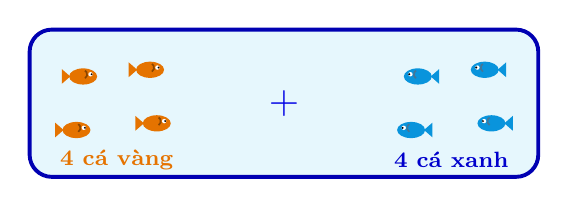
\begin{tikzpicture}[scale=0.85, baseline=(current bounding box.center)]
  % Bể kính viền xanh
  \draw[fill=cyan!10, draw=blue!70!black, line width=1.4pt, rounded corners=8pt] (-3.8,-1.1) rectangle (3.8,1.1);
  % 4 cá vàng bơi sang phải
  \VeChuCa[orange!90!black]{-3.0}{0.4}
  \VeChuCa[orange!90!black]{-2.0}{0.5}
  \VeChuCa[orange!90!black]{-3.1}{-0.4}
  \VeChuCa[orange!90!black]{-1.9}{-0.3}
  \node[font=\footnotesize\bfseries\color{orange!90!black}] at (-2.5,-0.85) {4 cá vàng};
  
  % Dấu cộng
  \node[font=\Large\bfseries\color{blue!90!black}] at (0,0) {$+$};
  
  % 4 cá xanh bơi sang trái
  \VeChuCaBoiTrai[cyan!80!blue]{2.0}{0.4}
  \VeChuCaBoiTrai[cyan!80!blue]{3.0}{0.5}
  \VeChuCaBoiTrai[cyan!80!blue]{1.9}{-0.4}
  \VeChuCaBoiTrai[cyan!80!blue]{3.1}{-0.3}
  \node[font=\footnotesize\bfseries\color{blue!80!black}] at (2.5,-0.85) {4 cá xanh};
\end{tikzpicture}
\end{center}
\choice
{$7$ chú cá}
{\True $8$ chú cá}
{$9$ chú cá}
{$10$ chú cá}
\loigiai{
Có tất cả: $4 + 4 = 8$ chú cá.\\
\textbf{Đáp án của câu hỏi là B}
}
\end{ex}

% --- CÂU 3 ---
\begin{ex} %[1D3H10]
Đĩa bên trái có 5 quả dâu tây đỏ, đĩa bên phải rỗng không có quả nào. Hỏi có tất cả bao nhiêu quả dâu tây?
\begin{center}
\begin{tikzpicture}[scale=0.85, baseline=(current bounding box.center)]
  % Đĩa trái 5 quả
  \draw[fill=yellow!20, draw=orange!80!black, line width=1.2pt] (-2.2,-0.2) ellipse (1.6cm and 0.5cm);
  \foreach \x in {-3.2, -2.7, -2.2, -1.7, -1.2} {
    \VeQuaTaoDo{\x}{0.05}
  }
  \node[below=3pt, font=\small\bfseries\color{red!85!black}] at (-2.2,-0.35) {5 quả dâu};
  
  % Dấu cộng
  \node[font=\LARGE\bfseries\color{blue!90!black}] at (0,0.1) {$+$};
  
  % Đĩa phải 0 quả
  \draw[fill=yellow!20, draw=orange!80!black, line width=1.2pt] (2.2,-0.2) ellipse (1.6cm and 0.5cm);
  \node[font=\small\itshape\color{gray}] at (2.2,0.1) {(Đĩa trống)};
  \node[below=3pt, font=\small\bfseries\color{gray!80!black}] at (2.2,-0.35) {0 quả};
\end{tikzpicture}
\end{center}
\choice
{$0$ quả}
{$6$ quả}
{\True $5$ quả}
{$4$ quả}
\loigiai{
Một số cộng với 0 bằng chính số đó: $5 + 0 = 5$ quả.\\
\textbf{Đáp án của câu hỏi là C}
}
\end{ex}

% --- CÂU 4 ---
\begin{ex} %[1D3H10]
Khung mười ô (Ten-frame) dưới đây có 6 chấm tròn màu đỏ và 3 chấm tròn màu xanh. Hỏi có tất cả bao nhiêu chấm tròn?
\begin{center}
\begin{tikzpicture}[scale=0.75, baseline=(current bounding box.center)]
  % Khung 10 ô (2 hàng 5 cột)
  \draw[fill=white, draw=blue!85!black, line width=1.5pt] (-2.75,-1.1) rectangle (2.75,1.1);
  \foreach \x in {-1.65, -0.55, 0.55, 1.65} {
    \draw[line width=1pt, blue!70!black] (\x,-1.1) -- (\x,1.1);
  }
  \draw[line width=1pt, blue!70!black] (-2.75,0) -- (2.75,0);
  
  % Hàng 1: 5 chấm đỏ
  \foreach \x in {-2.2, -1.1, 0, 1.1, 2.2} {
    \fill[red!85!black] (\x,0.55) circle (0.35cm);
  }
  % Hàng 2: 1 chấm đỏ, 3 chấm xanh
  \fill[red!85!black] (-2.2,-0.55) circle (0.35cm);
  \fill[cyan!75!blue] (-1.1,-0.55) circle (0.35cm);
  \fill[cyan!75!blue] (0,-0.55) circle (0.35cm);
  \fill[cyan!75!blue] (1.1,-0.55) circle (0.35cm);
  
  \node[below=5pt, font=\small\bfseries\color{blue!90!black}] at (0,-1.2) {6 chấm đỏ $+$ 3 chấm xanh};
\end{tikzpicture}
\end{center}
\choice
{$8$ chấm}
{$10$ chấm}
{\True $9$ chấm}
{$7$ chấm}
\loigiai{
Phép tính gộp: $6 + 3 = 9$ chấm tròn.\\
\textbf{Đáp án của câu hỏi là C}
}
\end{ex}

\newpage
% --- CÂU 5 ---
\begin{ex} %[1D3H10]
Dải băng số gồm 7 ô màu vàng và 3 ô màu xanh như hình vẽ. Tổng số ô của cả dải băng là bao nhiêu?
\begin{center}
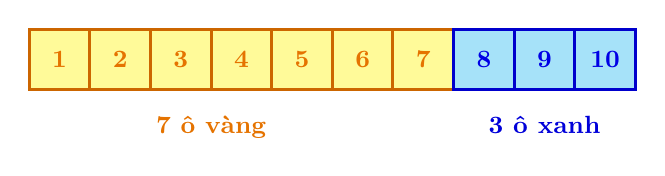
\begin{tikzpicture}[scale=0.7, baseline=(current bounding box.center)]
  % 7 ô vàng
  \foreach \i in {0,1,2,3,4,5,6} {
    \draw[fill=yellow!40, draw=orange!80!black, line width=1.1pt] (\i*1.1 - 5.5, -0.55) rectangle (\i*1.1 - 4.4, 0.55);
    \node[font=\small\bfseries\color{orange!90!black}] at (\i*1.1 - 4.95, 0) {\pgfmathparse{int(\i+1)}\pgfmathresult};
  }
  % 3 ô xanh
  \foreach \i in {0,1,2} {
    \draw[fill=cyan!35, draw=blue!80!black, line width=1.1pt] (\i*1.1 + 2.2, -0.55) rectangle (\i*1.1 + 3.3, 0.55);
    \node[font=\small\bfseries\color{blue!90!black}] at (\i*1.1 + 2.75, 0) {\pgfmathparse{int(\i+8)}\pgfmathresult};
  }
  \node[below=4pt, font=\small\bfseries\color{orange!90!black}] at (-2.2,-0.65) {7 ô vàng};
  \node[below=4pt, font=\small\bfseries\color{blue!85!black}] at (3.85,-0.65) {3 ô xanh};
\end{tikzpicture}
\end{center}
\choice
{$9$ ô}
{$8$ ô}
{$6$ ô}
{\True $10$ ô}
\loigiai{
Số ô của cả dải băng là: $7 + 3 = 10$ ô.\\
\textbf{Đáp án của câu hỏi là D}
}
\end{ex}

% --- CÂU 6 ---
\begin{ex} %[1D3H10]
Trong hộp có 4 viên kẹo cam. Cần thêm mấy viên kẹo xanh nữa để trong hộp có tất cả 7 viên kẹo?
\begin{center}
\begin{tikzpicture}[scale=0.8, baseline=(current bounding box.center)]
  % Hộp kẹo
  \draw[fill=purple!8, draw=purple!80!black, line width=1.3pt, rounded corners=6pt] (-3.8,-1.1) rectangle (3.8,1.1);
  % 4 viên kẹo cam
  \VeVienKeo[orange!90!black]{-2.7}{0}
  \VeVienKeo[orange!90!black]{-1.7}{0}
  \VeVienKeo[orange!90!black]{-0.7}{0}
  \VeVienKeo[orange!90!black]{0.3}{0}
  \node[below=3pt, font=\footnotesize\bfseries\color{orange!90!black}] at (-1.2,-0.55) {Có sẵn: 4 viên};
  
  % Vách ngăn nét đứt
  \draw[dashed, line width=1pt, gray!60] (1.1,-0.9) -- (1.1,0.9);
  
  % Dấu hỏi chấm kẹo cần thêm
  \node[font=\Large\bfseries\color{magenta!85!black}] at (2.4,0.1) {? viên};
  \node[below=3pt, font=\footnotesize\bfseries\color{magenta!85!black}] at (2.4,-0.55) {Thêm vào để được 7};
\end{tikzpicture}
\end{center}
\choice
{$2$ viên}
{$4$ viên}
{$5$ viên}
{\True $3$ viên}
\loigiai{
Phép tính: $4 + 3 = 7$. Cần thêm \textbf{3 viên kẹo}.\\
\textbf{Đáp án của câu hỏi là D}
}
\end{ex}

% --- CÂU 7 ---
\begin{ex} %[1D3V10]
An có 3 viên kẹo dâu, Bình cho An thêm 4 viên kẹo dâu nữa như hình vẽ. An có tất cả bao nhiêu viên kẹo?
\begin{center}
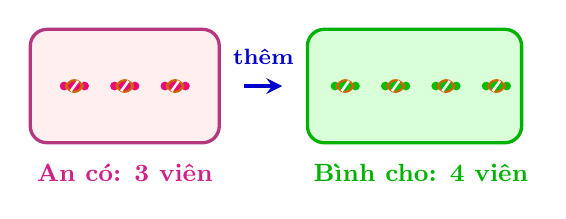
\begin{tikzpicture}[scale=0.8, baseline=(current bounding box.center)]
  % An có 3 viên
  \draw[fill=pink!25, draw=magenta!70!black, line width=1.2pt, rounded corners=6pt] (-3.7,-0.9) rectangle (-0.7,0.9);
  \VeVienKeo[magenta!80!red]{-3.0}{0}
  \VeVienKeo[magenta!80!red]{-2.2}{0}
  \VeVienKeo[magenta!80!red]{-1.4}{0}
  \node[below=3pt, font=\small\bfseries\color{magenta!85!black}] at (-2.2,-0.95) {An có: 3 viên};
  
  % Mũi tên thêm vào
  \draw[->, >=stealth, line width=1.5pt, blue!80!black] (-0.3,0) -- (0.3,0);
  \node[above=2pt, font=\footnotesize\bfseries\color{blue!80!black}] at (0,0.1) {thêm};
  
  % Bình cho thêm 4 viên
  \draw[fill=green!15, draw=green!70!black, line width=1.2pt, rounded corners=6pt] (0.7,-0.9) rectangle (4.1,0.9);
  \VeVienKeo[green!75!black]{1.3}{0}
  \VeVienKeo[green!75!black]{2.1}{0}
  \VeVienKeo[green!75!black]{2.9}{0}
  \VeVienKeo[green!75!black]{3.7}{0}
  \node[below=3pt, font=\small\bfseries\color{green!70!black}] at (2.5,-0.95) {Bình cho: 4 viên};
\end{tikzpicture}
\end{center}
\choice
{$6$ viên}
{\True $7$ viên}
{$8$ viên}
{$9$ viên}
\loigiai{
An có tất cả: $3 + 4 = 7$ viên kẹo.\\
\textbf{Đáp án của câu hỏi là B}
}
\end{ex}

% --- CÂU 8 ---
\begin{ex} %[1D3V10]
Trên cành cây có 5 chú chim sẻ đang đậu, có thêm 3 chú chim sẻ khác đang bay tới đậu cùng. Hỏi trên cây có tất cả bao nhiêu chú chim?
\begin{center}
\begin{tikzpicture}[scale=0.85, baseline=(current bounding box.center)]
  % Cành cây nâu
  \draw[brown!80!black, line width=4pt, line cap=round] (-3.8,-0.3) -- (1.5,-0.3);
  \draw[brown!80!black, line width=2.5pt, line cap=round] (0.2,-0.3) -- (0.8,0.2);
  % Lá cây xanh
  \fill[green!70!black] (-3.2,-0.15) ellipse (0.2cm and 0.1cm);
  \fill[green!70!black] (0.85,0.25) ellipse (0.2cm and 0.1cm);
  
  % 5 chú chim đậu
  \VeChuChimDau{-3.0}{0.05}
  \VeChuChimDau{-2.1}{0.05}
  \VeChuChimDau{-1.2}{0.05}
  \VeChuChimDau{-0.3}{0.05}
  \VeChuChimDau{0.6}{0.05}
  \node[below=4pt, font=\small\bfseries\color{blue!85!black}] at (-1.2,-0.4) {Đang đậu: 5 chú chim};
  
  % 3 chú chim đang bay tới
  \VeChuChimBay{2.2}{0.8}
  \VeChuChimBay{3.1}{0.4}
  \VeChuChimBay{2.4}{-0.1}
  \draw[->, >=stealth, dashed, line width=1.1pt, orange!90!black] (2.8,0.9) -- (1.6,0.3);
  \node[below=4pt, font=\small\bfseries\color{orange!90!black}] at (2.7,-0.4) {Bay tới: 3 chú chim};
\end{tikzpicture}
\end{center}
\choice
{\True $8$ chú chim}
{$7$ chú chim}
{$9$ chú chim}
{$10$ chú chim}
\loigiai{
Có tất cả: $5 + 3 = 8$ chú chim.\\
\textbf{Đáp án của câu hỏi là A}
}
\end{ex}

\newpage
% --- CÂU 9 ---
\begin{ex} %[1D3V10]
Có 3 đĩa quả: đĩa cam có 2 quả, đĩa táo có 3 quả và đĩa dâu có 4 quả. Tổng số quả trong 3 đĩa là bao nhiêu?
\begin{center}
\begin{tikzpicture}[scale=0.8, baseline=(current bounding box.center)]
  % Đĩa 1: 2 quả cam
  \draw[fill=orange!15, draw=orange!80!black, line width=1.1pt] (-3.2,-0.25) ellipse (1.1cm and 0.35cm);
  \VeQuaTaoXanh{-3.6}{0}
  \VeQuaTaoXanh{-2.8}{0}
  \node[below=2pt, font=\footnotesize\bfseries\color{green!70!black}] at (-3.2,-0.35) {2 quả};
  
  % Dấu +
  \node[font=\Large\bfseries\color{blue!90!black}] at (-1.8,0) {$+$};
  
  % Đĩa 2: 3 quả táo
  \draw[fill=orange!15, draw=orange!80!black, line width=1.1pt] (-0.4,-0.25) ellipse (1.2cm and 0.38cm);
  \VeQuaTaoDo{-0.9}{0}
  \VeQuaTaoDo{-0.4}{0}
  \VeQuaTaoDo{0.1}{0}
  \node[below=2pt, font=\footnotesize\bfseries\color{red!80!black}] at (-0.4,-0.35) {3 quả};
  
  % Dấu +
  \node[font=\Large\bfseries\color{blue!90!black}] at (1.0,0) {$+$};
  
  % Đĩa 3: 4 quả
  \draw[fill=orange!15, draw=orange!80!black, line width=1.1pt] (2.6,-0.25) ellipse (1.3cm and 0.4cm);
  \VeQuaTaoDo{1.9}{0}
  \VeQuaTaoDo{2.4}{0}
  \VeQuaTaoDo{2.9}{0}
  \VeQuaTaoDo{3.4}{0}
  \node[below=2pt, font=\footnotesize\bfseries\color{red!80!black}] at (2.6,-0.35) {4 quả};
\end{tikzpicture}
\end{center}
\choice
{\True $9$ quả}
{$8$ quả}
{$10$ quả}
{$7$ quả}
\loigiai{
Phép tính: $2 + 3 + 4 = 5 + 4 = 9$ quả.\\
\textbf{Đáp án của câu hỏi là A}
}
\end{ex}

% --- CÂU 10 ---
\begin{ex} %[1D3V10]
Quan sát chiếc cân đĩa thăng bằng ở hình dưới. So sánh hai vế phép tính $3 + 5$ và $4 + 4$:
\begin{center}
\begin{tikzpicture}[scale=0.8, baseline=(current bounding box.center)]
  % Trụ cân ở giữa
  \fill[gray!80!black] (-0.25,-1.2) rectangle (0.25,0);
  \fill[blue!90!black] (0,0) circle (0.15cm);
  \draw[fill=gray!60, draw=gray!90!black, line width=1pt] (-1.2,-1.4) rectangle (1.2,-1.15);
  % Đòn cân nằm ngang thăng bằng
  \draw[line width=2.5pt, blue!90!black] (-3.0,0) -- (3.0,0);
  
  % Đĩa cân trái (3+5)
  \draw[line width=1pt, gray!70!black] (-3.0,0) -- (-3.8,-0.6);
  \draw[line width=1pt, gray!70!black] (-3.0,0) -- (-2.2,-0.6);
  \draw[fill=orange!25, draw=orange!90!black, line width=1.2pt] (-3.0,-0.6) ellipse (1.1cm and 0.25cm);
  \node[above=2pt, font=\small\bfseries\color{blue!90!black}] at (-3.0,-0.55) {$3 + 5 = 8$};
  
  % Đĩa cân phải (4+4)
  \draw[line width=1pt, gray!70!black] (3.0,0) -- (2.2,-0.6);
  \draw[line width=1pt, gray!70!black] (3.0,0) -- (3.8,-0.6);
  \draw[fill=orange!25, draw=orange!90!black, line width=1.2pt] (3.0,-0.6) ellipse (1.1cm and 0.25cm);
  \node[above=2pt, font=\small\bfseries\color{blue!90!black}] at (3.0,-0.55) {$4 + 4 = 8$};
  
  \node[below=4pt, font=\small\bfseries\color{purple!85!black}] at (0,-1.4) {Cân thăng bằng: $3 + 5 \dots 4 + 4$};
\end{tikzpicture}
\end{center}
\choice
{$>$}
{\True $=$}
{$<$}
{Không so sánh được}
\loigiai{
Ta có $3 + 5 = 8$ và $4 + 4 = 8$. Vì $8 = 8$ nên dấu thích hợp là dấu $=$.\\
\textbf{Đáp án của câu hỏi là B}
}
\end{ex}

% --- CÂU 11 ---
\begin{ex} %[1D3V10]
Mẹ để 5 quả trứng gà trong rổ vàng và 5 quả trứng vịt trong rổ xanh. Hỏi cả hai rổ có tất cả bao nhiêu quả trứng?
\begin{center}
\begin{tikzpicture}[scale=0.8, baseline=(current bounding box.center)]
  % Rổ 1: 5 quả trứng gà
  \draw[fill=yellow!20, draw=orange!80!black, line width=1.3pt, rounded corners=6pt] (-4.0,-0.8) rectangle (-0.6,0.8);
  \foreach \i in {0,1,2,3,4} {
    \fill[orange!35, draw=orange!80!black, line width=0.8pt] (\i*0.65-3.6, 0) ellipse (0.24cm and 0.32cm);
  }
  \node[below=3pt, font=\small\bfseries\color{orange!90!black}] at (-2.3,-0.85) {5 quả trứng gà};
  
  % Dấu +
  \node[font=\LARGE\bfseries\color{blue!90!black}] at (0,0) {$+$};
  
  % Rổ 2: 5 quả trứng vịt
  \draw[fill=cyan!15, draw=blue!80!black, line width=1.3pt, rounded corners=6pt] (0.6,-0.8) rectangle (4.0,0.8);
  \foreach \i in {0,1,2,3,4} {
    \fill[white, draw=blue!70!black, line width=0.8pt] (\i*0.65+1.0, 0) ellipse (0.24cm and 0.32cm);
  }
  \node[below=3pt, font=\small\bfseries\color{blue!85!black}] at (2.3,-0.85) {5 quả trứng vịt};
\end{tikzpicture}
\end{center}
\choice
{$9$ quả}
{$8$ quả}
{\True $10$ quả}
{$7$ quả}
\loigiai{
Số quả trứng có tất cả là: $5 + 5 = 10$ quả trứng.\\
\textbf{Đáp án của câu hỏi là C}
}
\end{ex}

% --- CÂU 12 ---
\begin{ex} %[1D3C10]
Quan sát sơ đồ tính dưới đây. Số thích hợp điền vào dấu hỏi chấm là bao nhiêu?
\begin{center}
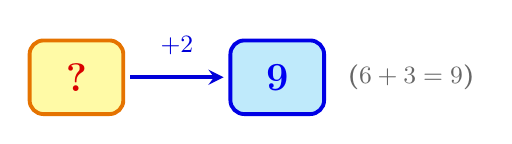
\begin{tikzpicture}[scale=0.85, baseline=(current bounding box.center)]
  % Ô hỏi chấm
  \draw[fill=yellow!35, draw=orange!90!black, line width=1.4pt, rounded corners=5pt] (-3.2,-0.55) rectangle (-1.8,0.55);
  \node[font=\Large\bfseries\color{red!85!black}] at (-2.5,0) {?};
  
  % Mũi tên cộng 2
  \draw[->, >=stealth, line width=1.4pt, blue!85!black] (-1.7,0) -- (-0.3,0);
  \node[above=2pt, font=\small\bfseries\color{blue!85!black}] at (-1.0,0.1) {$+ 2$};
  
  % Ô kết quả 9
  \draw[fill=cyan!25, draw=blue!90!black, line width=1.4pt, rounded corners=5pt] (-0.2,-0.55) rectangle (1.2,0.55);
  \node[font=\Large\bfseries\color{blue!95!black}] at (0.5,0) {9};
  
  % Gợi ý
  \node[font=\small\bfseries\color{gray!80!black}] at (2.5,0) {($6 + 3 = 9$)};
\end{tikzpicture}
\end{center}
\choice
{\True $7$}
{$6$}
{$8$}
{$9$}
\loigiai{
Ta có: $7 + 2 = 9$. Vậy số cần tìm là \textbf{7}.\\
\textbf{Đáp án của câu hỏi là A}
}
\end{ex}

\newpage
% =========================================================================
% PHẦN 2: TRẮC NGHIỆM ĐÚNG SAI (2 CÂU)
% =========================================================================
\textbf{Phần 2. Trắc nghiệm đúng sai}
\setcounterpageref{ex}{0}

% --- CÂU 13 ---
\begin{ex} %[1D3H10]
Quan sát các phép tính cộng trong phạm vi 10 và xét tính đúng sai của từng câu:
\begin{center}
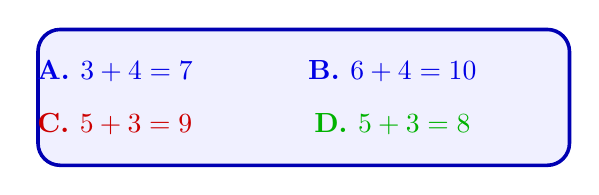
\begin{tikzpicture}[scale=0.75, baseline=(current bounding box.center)]
  % Bảng tính xinh xắn
  \draw[fill=blue!6, draw=blue!70!black, line width=1.3pt, rounded corners=8pt] (-4.5,-1.15) rectangle (4.5,1.15);
  % 4 phép tính
  \node[font=\normalsize\bfseries\color{blue!90!black}] at (-3.2,0.45) {A. $3 + 4 = 7$};
  \node[font=\normalsize\bfseries\color{blue!90!black}] at (1.5,0.45) {B. $6 + 4 = 10$};
  \node[font=\normalsize\bfseries\color{red!80!black}] at (-3.2,-0.45) {C. $5 + 3 = 9$};
  \node[font=\normalsize\bfseries\color{green!70!black}] at (1.5,-0.45) {D. $5 + 3 = 8$};
\end{tikzpicture}
\end{center}
\choiceTF
{\True $3 + 4 = 7$ là phép tính đúng.}
{\True $6 + 4 = 10$ là phép tính đúng.}
{Phép tính $5 + 3 = 9$ là phép tính đúng.}
{\True Kết quả đúng của $5 + 3$ phải là $8$.}
\loigiai{
\begin{itemize}
    \item a) \textbf{Đúng}: $3 + 4 = 7$.
    \item b) \textbf{Đúng}: $6 + 4 = 10$.
    \item c) \textbf{Sai}: $5 + 3 = 8$, không phải bằng $9$.
    \item d) \textbf{Đúng}: $5 + 3 = 8$.
\end{itemize}
}
\end{ex}

% --- CÂU 14 ---
\begin{ex} %[1D3V10]
Bạn Lan cắm 4 bông hoa hồng đỏ và 5 bông hoa cúc vàng vào bình hoa như hình vẽ:
\begin{center}
\begin{tikzpicture}[scale=0.8, baseline=(current bounding box.center)]
  % Bình hoa
  \draw[fill=cyan!20, draw=blue!85!black, line width=1.4pt] (-0.8,-1.2) -- (0.8,-1.2) -- (1.1,0) -- (0.6,0.3) -- (-0.6,0.3) -- (-1.1,0) -- cycle;
  \node[font=\tiny\bfseries\color{blue!80!black}] at (0,-0.5) {Bình hoa};
  
  % 4 hoa đỏ
  \VeBongHoaNho[red!85!black]{-1.3,}{0.8}
  \VeBongHoaNho[red!85!black]{-0.6}{1.3}
  \VeBongHoaNho[red!85!black]{-0.8}{0.7}
  \VeBongHoaNho[red!85!black]{-0.2}{1.6}
  \node[font=\footnotesize\bfseries\color{red!85!black}] at (-2.3,1.1) {4 hoa đỏ};
  \draw[->, >=stealth, red!85!black, line width=0.8pt] (-1.6,1.1) -- (-1.1,1.1);
  
  % 5 hoa vàng
  \VeBongHoaNho[yellow!90!orange]{0.3}{1.5}
  \VeBongHoaNho[yellow!90!orange]{0.8}{1.1}
  \VeBongHoaNho[yellow!90!orange]{1.2}{0.7}
  \VeBongHoaNho[yellow!90!orange]{0.6}{0.7}
  \VeBongHoaNho[yellow!90!orange]{1.4}{1.3}
  \node[font=\footnotesize\bfseries\color{orange!90!black}] at (2.4,1.1) {5 hoa vàng};
  \draw[->, >=stealth, orange!90!black, line width=0.8pt] (1.7,1.1) -- (1.2,1.1);
\end{tikzpicture}
\end{center}
Xét tính đúng sai của các câu sau:
\choiceTF
{\True Lan có tất cả 9 bông hoa ($4 + 5 = 9$).}
{\True Số hoa vàng nhiều hơn số hoa đỏ là 1 bông ($5 - 4 = 1$).}
{Nếu cắm thêm 2 bông hoa đỏ nữa thì Lan có tất cả 10 bông hoa.}
{\True Khi cắm thêm 2 bông hoa đỏ nữa thì Lan có tất cả 11 bông hoa.}
\loigiai{
\begin{itemize}
    \item a) \textbf{Đúng}: Tổng số hoa là $4 + 5 = 9$ bông hoa.
    \item b) \textbf{Đúng}: $5 - 4 = 1$ bông.
    \item c) \textbf{Sai}: $9 + 2 = 11$ bông hoa, không phải 10.
    \item d) \textbf{Đúng}: Khi cắm thêm 2 bông hoa đỏ thì $9 + 2 = 11$ bông hoa.
\end{itemize}
}
\end{ex}

% =========================================================================
% PHẦN 3: TRẢ LỜI NGẮN (6 CÂU)
% =========================================================================
\textbf{Phần 3. Trả lời ngắn (Quan sát hình vẽ và điền số thích hợp)}
\setcounterpageref{ex}{0}

% --- CÂU 15 ---
\begin{ex} %[1D3H10]
Quan sát hình vẽ và tính kết quả của phép cộng $3 + 5$:
\begin{center}
\begin{tikzpicture}[scale=0.75, baseline=(current bounding box.center)]
  % Hàng trên: 3 ngôi sao vàng
  \foreach \i in {0,1,2} {
    \node[star, star points=5, star point ratio=2.25, fill=yellow!90!orange, draw=orange!90!black, line width=0.8pt, minimum size=0.75cm] at (\i*1.2 - 1.2, 0.6) {};
  }
  \node[font=\small\bfseries\color{orange!90!black}] at (-2.3,0.6) {3 sao:};
  
  % Hàng dưới: 5 ngôi sao xanh
  \foreach \i in {0,1,2,3,4} {
    \node[star, star points=5, star point ratio=2.25, fill=cyan!75!blue, draw=blue!90!black, line width=0.8pt, minimum size=0.75cm] at (\i*1.2 - 2.4, -0.6) {};
  }
  \node[font=\small\bfseries\color{blue!85!black}] at (-3.5,-0.6) {5 sao:};
\end{tikzpicture}
\end{center}
\shortans{8}
\loigiai{
\textbf{Đáp số:} $8$\\
$3 + 5 = 8$.
}
\end{ex}

% --- CÂU 16 ---
\begin{ex} %[1D3H10]
Quan sát thanh mười ô dưới đây gồm 6 chấm tròn màu cam và 4 chấm tròn màu xanh. Cả thanh có bao nhiêu chấm tròn?
\begin{center}
\begin{tikzpicture}[scale=0.75, baseline=(current bounding box.center)]
  % 10 ô liên tiếp
  \foreach \i in {0,1,2,3,4,5} {
    \draw[fill=orange!25, draw=orange!85!black, line width=1.1pt] (\i*0.9 - 4.5, -0.45) rectangle (\i*0.9 - 3.6, 0.45);
    \fill[orange!90!black] (\i*0.9 - 4.05, 0) circle (0.26cm);
  }
  \foreach \i in {0,1,2,3} {
    \draw[fill=cyan!25, draw=blue!85!black, line width=1.1pt] (\i*0.9 + 0.9, -0.45) rectangle (\i*0.9 + 1.8, 0.45);
    \fill[blue!85!black] (\i*0.9 + 1.35, 0) circle (0.26cm);
  }
  \node[below=4pt, font=\small\bfseries\color{orange!90!black}] at (-1.8,-0.5) {6 chấm cam};
  \node[below=4pt, font=\small\bfseries\color{blue!85!black}] at (2.7,-0.5) {4 chấm xanh};
\end{tikzpicture}
\end{center}
\shortans{10}
\loigiai{
\textbf{Đáp số:} $10$\\
$6 + 4 = 10$.
}
\end{ex}

\newpage
% --- CÂU 17 ---
\begin{ex} %[1D3V10]
Có 3 đĩa bánh: đĩa thứ nhất có 1 cái bánh, đĩa thứ hai có 4 cái bánh, đĩa thứ ba có 5 cái bánh như hình vẽ. Hỏi có tất cả bao nhiêu cái bánh?
\begin{center}
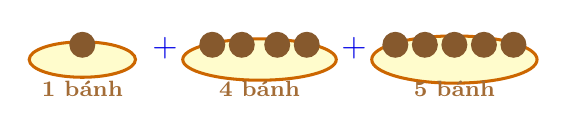
\begin{tikzpicture}[scale=0.75, baseline=(current bounding box.center)]
  % Đĩa 1 (1 bánh)
  \draw[fill=yellow!20, draw=orange!80!black, line width=1.1pt] (-3.4,-0.2) ellipse (0.9cm and 0.3cm);
  \fill[brown!70!black] (-3.4,0.05) circle (0.22cm);
  \node[below=2pt, font=\footnotesize\bfseries\color{brown!85!black}] at (-3.4,-0.3) {1 bánh};
  
  \node[font=\large\bfseries\color{blue!90!black}] at (-2.0,0) {$+$};
  
  % Đĩa 2 (4 bánh)
  \draw[fill=yellow!20, draw=orange!80!black, line width=1.1pt] (-0.4,-0.2) ellipse (1.3cm and 0.35cm);
  \foreach \x in {-1.2, -0.7, -0.1, 0.4} {
    \fill[brown!70!black] (\x,0.05) circle (0.22cm);
  }
  \node[below=2pt, font=\footnotesize\bfseries\color{brown!85!black}] at (-0.4,-0.3) {4 bánh};
  
  \node[font=\large\bfseries\color{blue!90!black}] at (1.2,0) {$+$};
  
  % Đĩa 3 (5 bánh)
  \draw[fill=yellow!20, draw=orange!80!black, line width=1.1pt] (2.9,-0.2) ellipse (1.4cm and 0.4cm);
  \foreach \x in {1.9, 2.4, 2.9, 3.4, 3.9} {
    \fill[brown!70!black] (\x,0.05) circle (0.22cm);
  }
  \node[below=2pt, font=\footnotesize\bfseries\color{brown!85!black}] at (2.9,-0.3) {5 bánh};
\end{tikzpicture}
\end{center}
\shortans{10}
\loigiai{
\textbf{Đáp số:} $10$\\
$1 + 4 + 5 = 5 + 5 = 10$ cái bánh.
}
\end{ex}

% --- CÂU 18 ---
\begin{ex} %[1D3V10]
Trong hộp có 4 chiếc bút chì. Bạn An bỏ thêm vào hộp một số chiếc bút chì để trong hộp có tất cả 9 chiếc bút chì. Hỏi An đã bỏ thêm vào bao nhiêu chiếc bút chì?
\begin{center}
\begin{tikzpicture}[scale=0.8, baseline=(current bounding box.center)]
  % Hộp bút
  \draw[fill=cyan!10, draw=blue!85!black, line width=1.3pt, rounded corners=6pt] (-3.8,-0.9) rectangle (3.8,0.9);
  % 4 bút chì có sẵn
  \foreach \i in {0,1,2,3} {
    \draw[fill=yellow!70!orange, draw=orange!90!black, line width=0.8pt] (\i*0.7-3.3,-0.6) rectangle (\i*0.7-2.9,0.5);
    \fill[brown!80!black] (\i*0.7-3.3,0.5) -- (\i*0.7-3.1,0.75) -- (\i*0.7-2.9,0.5) -- cycle;
    \fill[black] (\i*0.7-3.15,0.7) -- (\i*0.7-3.1,0.75) -- (\i*0.7-3.05,0.7) -- cycle;
  }
  \node[below=3pt, font=\footnotesize\bfseries\color{blue!90!black}] at (-2.25,-0.6) {Có sẵn 4 bút};
  
  % Vách ngăn
  \draw[dashed, line width=1pt, gray!60] (-0.3,-0.75) -- (-0.3,0.75);
  
  % Dấu hỏi chấm thêm vào
  \node[font=\Large\bfseries\color{red!85!black}] at (1.8,0.1) {Thêm: ? chiếc};
  \node[below=3pt, font=\footnotesize\bfseries\color{red!85!black}] at (1.8,-0.55) {Để có tất cả 9 chiếc};
\end{tikzpicture}
\end{center}
\shortans{5}
\loigiai{
\textbf{Đáp số:} $5$\\
$9 - 4 = 5$ chiếc bút chì.
}
\end{ex}

% --- CÂU 19 ---
\begin{ex} %[1D3V10]
Dưới ao có 4 chú vịt đang bơi, trên bờ có 3 chú vịt nhảy xuống ao bơi cùng. Hỏi dưới ao có tất cả bao nhiêu chú vịt?
\begin{center}
\begin{tikzpicture}[scale=0.8, baseline=(current bounding box.center)]
  % Làn nước ao
  \draw[fill=cyan!15, draw=blue!70!black, line width=1.2pt, rounded corners=8pt] (-4.2,-1.05) rectangle (1.2,1.05);
  % 4 chú vịt dưới ao
  \VeChuVit{-3.4}{0.35}
  \VeChuVit{-2.1}{0.45}
  \VeChuVit{-3.2}{-0.45}
  \VeChuVit{-1.8}{-0.35}
  \node[below=3pt, font=\small\bfseries\color{blue!90!black}] at (-1.5,-0.75) {Dưới ao: 4 chú vịt};
  
  % Bờ cỏ
  \draw[fill=green!20, draw=green!70!black, line width=1.2pt, rounded corners=8pt] (1.6,-1.05) rectangle (4.4,1.05);
  % 3 chú vịt trên bờ
  \VeChuVit{2.4}{0.45}
  \VeChuVit{3.6}{0.35}
  \VeChuVit{3.0}{-0.35}
  \node[below=3pt, font=\small\bfseries\color{green!70!black}] at (3.0,-0.75) {Trên bờ: 3 chú};
  
  % Mũi tên nhảy xuống ao
  \draw[->, >=stealth, line width=1.5pt, blue!85!black] (1.8,0) to[out=150,in=30] (1.0,0);
\end{tikzpicture}
\end{center}
\shortans{7}
\loigiai{
\textbf{Đáp số:} $7$\\
$4 + 3 = 7$ chú vịt.
}
\end{ex}

% --- CÂU 20 ---
\begin{ex} %[1D3C10]
Trên bàn có 3 rổ quả: rổ thứ nhất có 2 quả táo đỏ, rổ thứ hai có 3 quả táo xanh, rổ thứ ba có 5 quả táo vàng. Tính nhanh tổng số quả táo trên bàn?
\begin{center}
\begin{tikzpicture}[scale=0.75, baseline=(current bounding box.center)]
  % Rổ 1: 2 quả đỏ
  \draw[fill=orange!15, draw=orange!80!black, line width=1.1pt] (-3.4,-0.2) ellipse (1.0cm and 0.35cm);
  \VeQuaTaoDo{-3.75}{0.05}
  \VeQuaTaoDo{-3.05}{0.05}
  \node[below=2pt, font=\footnotesize\bfseries\color{red!85!black}] at (-3.4,-0.35) {2 quả đỏ};
  
  \node[font=\large\bfseries\color{blue!90!black}] at (-1.9,0) {$+$};
  
  % Rổ 2: 3 quả xanh
  \draw[fill=orange!15, draw=orange!80!black, line width=1.1pt] (-0.4,-0.2) ellipse (1.2cm and 0.38cm);
  \VeQuaTaoXanh{-0.9}{0.05}
  \VeQuaTaoXanh{-0.4}{0.05}
  \VeQuaTaoXanh{0.1}{0.05}
  \node[below=2pt, font=\footnotesize\bfseries\color{green!70!black}] at (-0.4,-0.35) {3 quả xanh};
  
  \node[font=\large\bfseries\color{blue!90!black}] at (1.2,0) {$+$};
  
  % Rổ 3: 5 quả táo đỏ
  \draw[fill=orange!15, draw=orange!80!black, line width=1.1pt] (3.0,-0.2) ellipse (1.5cm and 0.42cm);
  \foreach \x in {1.9, 2.45, 3.0, 3.55, 4.1} {
    \VeQuaTaoDo{\x}{0.05}
  }
  \node[below=2pt, font=\footnotesize\bfseries\color{orange!90!black}] at (3.0,-0.35) {5 quả vàng};
\end{tikzpicture}
\end{center}
\shortans{10}
\loigiai{
\textbf{Đáp số:} $10$\\
Tính nhanh: $(2 + 3) + 5 = 5 + 5 = 10$ quả táo.
}
\end{ex}
